%\documentclass[manuscript]{geophysics}
%\usepackage[nomarkers]{endfloat}
% For a two-column format that looks like the final product, uncomment bellow
% and comment the two lines above
\documentclass[paper,twocolumn,twoside]{geophysics}

\usepackage{graphicx}
\usepackage{amsmath}

\newcommand{\vect}[1]{\mathbf{#1}}
\newcommand{\mat}[1]{\mathbf{#1}}
\newcommand{\comp}[1]{#1^{\alpha\beta}}
\newcommand{\norm}[1]{\left|\left|#1\right|\right|}

\begin{document}

\title{
    Tesseroids:
    command-line tools for
    gravity field forward modeling
    in spherical coordinates
}

% manuscript number
\ms{}

\address{
    \footnotemark[1]
    Universidade do Estado do Rio de Janeiro, Rio de Janeiro, Brazil,
    e-mail: leouieda@gmail.com;\\
    \footnotemark[2]
    Observat\'orio Nacional, Rio de Janeiro, Brazil;
}

\author{Leonardo Uieda\footnotemark[1]\footnotemark[2],
        Vanderlei C. Oliveira Jr\footnotemark[2],
        and
        Val\'eria C. F. Barbosa\footnotemark[2]}

\lefthead{Uieda et al.}
\righthead{Gravity forward modeling with Tesseroids}


\begin{abstract}
Lorem ipsum dolor sit amet, consectetur adipiscing elit. Nam eu dolor pretium,
egestas mauris sed, dapibus quam. Duis hendrerit mollis nunc a consequat. Nulla
et sem consectetur, interdum velit eget, aliquam ipsum. Praesent sagittis
tortor diam, sed ultrices magna ullamcorper vitae. Proin vitae orci augue.
Morbi dictum ligula gravida sem malesuada facilisis. Mauris nibh metus, cursus
eget imperdiet vitae, pretium at lorem. Praesent nisi mauris, pretium ut risus
fermentum, egestas tincidunt nibh. Mauris nulla orci, consequat eu pharetra
non, mattis ut urna. Mauris facilisis orci eros. Nam mattis non magna iaculis
consectetur. Morbi sodales dolor vitae felis sagittis, eget faucibus turpis
convallis. Nullam malesuada, mauris et ultricies rutrum, odio nulla gravida
nunc, ac volutpat eros lectus eget lacus. Integer venenatis velit vel justo
pellentesque, quis molestie sem vestibulum.
\end{abstract}

%%%%%%%%%%%%%%%%%%%%%%%%%%%%%%%%%%%%%%%%%%%%%%%%%%%%%%%%%%%%%%%%%%%%%%%%%%%%%%
\section{Introduction}

Citing articles in text \citet{Asgharzadeh2007} and with parenthesis
\citep{Braitenberg2011}.


%%%%%%%%%%%%%%%%%%%%%%%%%%%%%%%%%%%%%%%%%%%%%%%%%%%%%%%%%%%%%%%%%%%%%%%%%%%%%%
\section{Methodology}

The gravitational potential,
gravitational acceleration,
and Marussi (gravity gradient) tensor
caused by a homogeneous tesseroid
with density $\rho$
are \citep{Grombein2013}

\begin{equation}
    V(r,\phi,\lambda) = G \rho
        \int\limits_{\lambda_1}^{\lambda_2}
        \int\limits_{\phi_1}^{\phi_2}
        \int\limits_{r_1}^{r_2}
        \frac{1}{\ell} \kappa  dr' d\phi' d\lambda',
    \label{eq:tesspot}
\end{equation}
\begin{equation}
    g_{\alpha}(r,\phi,\lambda) = G \rho
        \int\limits_{\lambda_1}^{\lambda_2}
        \int\limits_{\phi_1}^{\phi_2}
        \int\limits_{r_1}^{r_2}
        \frac{\Delta_{\alpha}}{\ell^3} \kappa dr' d\phi' d\lambda'
        \ \ \ \alpha \in \{x,y,z\},
    \label{eq:tessgrav}
\end{equation}

\noindent
and

\begin{equation}
    g_{\alpha\beta}(r,\phi,\lambda) = G \rho
        \int\limits_{\lambda_1}^{\lambda_2}
        \int\limits_{\phi_1}^{\phi_2}
        \int\limits_{r_1}^{r_2}
        I_{\alpha\beta}
        dr' d\phi' d\lambda',
    \label{eq:tesstensor}
\end{equation}

\noindent
in which
$(\phi, \lambda, r)$ are
the latitude, longitude, and radius
coordinates of computation point P (Figure~\ref{fig:tesseroid}),
$\alpha,\beta \in \{x,y,z\}$
(the local coordinate system of point P),
and

\begin{eqnarray}
    I_{\alpha\beta} &=&
        \left(
            \frac{3\Delta_{\alpha} \Delta_{\beta}}{\ell^5} -
            \frac{\delta_{\alpha\beta}}{\ell^3}
        \right) \kappa, \\
    \Delta_x &=& r' K_{\phi} , \\
    \Delta_y &=& r' \cos \phi' \sin(\lambda' - \lambda) , \\
    \Delta_z &=& r' \cos \psi - r, \\
    \ell &=& \sqrt{r'^2 + r^2 - 2 r' r \cos \psi} , \\
    \cos\psi &=& \sin\phi\sin\phi' + \cos\phi\cos\phi'
                 \cos(\lambda' - \lambda) , \\
    K_{\phi} &=& \cos\phi\sin\phi' - \sin\phi\cos\phi'
                 \cos(\lambda' - \lambda), \\
    \kappa &=& {r'}^2 \cos \phi'.
\end{eqnarray}

\noindent
$\delta_{\alpha\beta}$ is the Kronecker delta,
i.e. $\delta_{\alpha\beta}=1$ if $\alpha=\beta$
and $\delta_{\alpha\beta}=0$ otherwise.

\begin{figure}
    \centering
    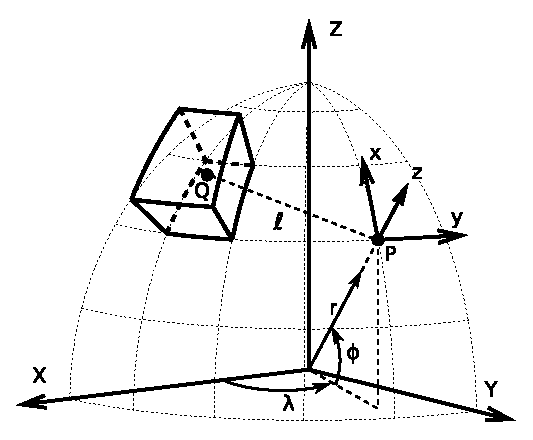
\includegraphics[width=\columnwidth]{figs/tesseroid}
    \caption{
        View of a tesseroid,
        the integration point $Q$,
        a geocentric coordinate system $(X, Y, Z)$,
        the computation $P$ and it's local coordinate system $(x, y, z)$.
        $r$, $\phi$, $\lambda$ are
        the radius, latitude, and longitude, respectively, of point $P$,
        and $\ell$ is the Cartesian distance between $P$ and $Q$.
    }
    \label{fig:tesseroid}
\end{figure}

The above integrals
have to be solved numerically
\citep{Wild-Pfeiffer2008}
and different approaches have been proposed.
\citet{Heck2007}
used a Taylor series expansion,
while \citet{Asgharzadeh2007}
used the Gauss-Legendre Quadrature (GLQ).
\citet{Wild-Pfeiffer2008} investigated
the use of both methods,
along with alternative mass elements,
and found the GLQ to be the most efficient method.
Therefore, we have opted to use
the 3D GLQ in our computations.

The Gauss-Legendre Quadrature
approximates the integral by
a weighted sum
\citep{Hildebrand1987},
e.g.

\begin{equation}
    \int\limits_a^b f(x) dx \approx
    \frac{b-a}{2}\sum\limits_{i=1}^N W_i f(x_i),
\end{equation}

\noindent
where the discretization points (nodes) $x_i$
are the roots of the $N$th order Legendre polynomial $P_N$
and the weights $W_i$ are \citep{Hildebrand1987}

\begin{equation}
    W_i = \frac{2}{(1 - x_i^2)(P'_N(x_i))^2}.
\end{equation}

The triple integrals in equations
\ref{eq:tesspot},
\ref{eq:tessgrav},
and
\ref{eq:tesstensor}
become

\begin{equation}
    V(r,\phi,\lambda) \approx
        A
        \sum\limits_{k=1}^{N^{\lambda}}
        \sum\limits_{j=1}^{N^{\phi}}
        \sum\limits_{i=1}^{N^r}
        W^r_i W^{\phi}_j W^{\lambda}_k
        \frac{1}{\ell} \kappa,
\end{equation}
\begin{equation}
    g_{\alpha}(r,\phi,\lambda) \approx
        A
        \sum\limits_{k=1}^{N^{\lambda}}
        \sum\limits_{j=1}^{N^{\phi}}
        \sum\limits_{i=1}^{N^r}
        W^r_i W^{\phi}_j W^{\lambda}_k
        \frac{\Delta_{\alpha}}{\ell^3} \kappa,
\end{equation}

\noindent
and

\begin{equation}
    g_{\alpha\beta}(r,\phi,\lambda) \approx
        A
        \sum\limits_{k=1}^{N^{\lambda}}
        \sum\limits_{j=1}^{N^{\phi}}
        \sum\limits_{i=1}^{N^r}
        W^r_i W^{\phi}_j W^{\lambda}_k
        I_{\alpha\beta},
\end{equation}

\noindent
where

\begin{equation}
    A = G \rho
    \frac{(\lambda_2 - \lambda_1)(\phi_2 - \phi_1)(r_2 - r_1)}{8},
\end{equation}

\noindent
$W_i^r$, $W_j^{\phi}$, and $W_k^{\lambda}$
are the weights
and $N^r$, $N^{\phi}$, and $N^{\lambda}$
are the number of nodes
for the radial, latitudinal, and longitudinal dimensions, respectively.

The accuracy of the numerical integration
using the GLQ
was investigated by \citet{Ku1977}
for the case of the right-rectangular prism.
\citet{Ku1977} found that the accuracy
depends on the ratio between
the average distance between GLQ nodes
and the distance to the observation point P.
As a rule-of-thumb,
\citet{Ku1977} suggests that
the distance between nodes
should not be greater than
the distance to point P.
\citet{Li2011} devised a scheme that
recursively subdivides the tesseroids
into smaller ones,
effectively decreasing the distance between nodes.
This scheme guarantees that
the rule-of-thumb is not violated.
Hence,
optimal accuracy of the numerical integration
is achieved automatically.

We use a modified version
of the recursive scheme of \citet{Li2011}.
We fix the number of nodes in the GLQ
$N^\lambda=N^\phi=N^r=2$.
In this case, the maximum distance between nodes
is approximately the largest dimension of the tesseroid ($L$)
\citep{Wild-Pfeiffer2008}.
For a computation point $P$
at a distance $d$ from
the center of the top face of the tesseroid
(Figure~\ref{fig:ratio}a),
the tesseroid is divided in eight parts if

\begin{equation}
    \frac{d}{L} < R,
    \label{eq:ratio}
\end{equation}

\noindent
where $R$ is the minimum distance/size ratio desired.
In case the tesseroid is divided,
the inequality in equation \ref{eq:ratio}
is checked for each of the eight parts.
This process is repeated recursively
until no divisions are required,
ensuring that equation \ref{eq:ratio}
holds for all tesseroids created.
The gravitational effect
of the original tesseroid
is then calculated as
the sum of the effect
of the smaller tesseroids.

The rule-of-thumb of \citet{Ku1977}
used by \citet{Li2011}
is equivalent to setting $R=1$.
Figure~\ref{fig:ratio}
illustrates the subdivision of a tesseroid
(Figure~\ref{fig:ratio}a)
for computation point $P$
using increasing values of $R$.
Note that increasing $R$
results is a finer division of the tesseroid
around the computation point
and thus a more accurate GLQ integration.
However, higher values of $R$
also result in
larger computation times.
For example,
the tesseroid in Figure~\ref{fig:ratio}a
is replaced by
50 tesseroids for $R=0.5$ (Figure~\ref{fig:ratio}b),
344 tesseroids for $R=1$ (Figure~\ref{fig:ratio}c),
and 2472 tesseroids for  $R=2$ (Figure~\ref{fig:ratio}d).

\begin{figure}
    \centering
    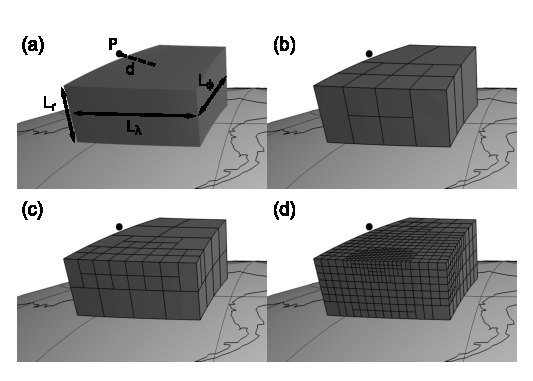
\includegraphics[width=\columnwidth]{figs/tesseroid-split}
    \caption{
        Adaptive discretization
        of the tesseroid shown in (a)
        for a computation point P
        using $R$ equal to
        (b) 0.5, (c) 1, and (d) 2.
        $d$ is the distance between
        the center of the top face of the tesseroid
        and $P$.
        $L$ is the largest dimension of the tesseroid.
    }
    \label{fig:ratio}
\end{figure}

Clearly,
there is need to determine
an optimal value of $R$
that yields the desired accuracy
in the GLQ integration.
In the following section,
we compare the computed gravitational effects
of a tesseroid model
with that of a spherical half-shell
(Figure~\ref{fig:shell}),
for which exist analytical expressions.


\subsection{Comparison with a spherical half-shell}

The gravitational potential,
gravitational attraction,
and
Marussi (gravity gradient) tensor
caused by the homogeneous spherical half-shell
shown in Figure~\ref{fig:shell}
at a computation point
$P = (\lambda=90^\circ, \phi=0^\circ, r=r_2+h)$
are

\begin{equation}
    V(h) = 2\pi G \rho \left[
        \dfrac{l^3 + {r'}^3}{3(r_2 + h)} - 0.5 {r'}^2 \right]
         \Biggr \rvert_{r'=r_1}^{r'=r_2},
    \label{eq:shellpot}
\end{equation}
\begin{equation}
    g_z(h) = 2\pi G \rho \left[
        \dfrac{l^3 + {r'}^3}{3(r_2 + h)^2} - l \right]
        \Biggr \rvert_{r'=r_1}^{r'=r_2},
    \label{eq:shellgz}
\end{equation}
\begin{equation}
    g_{xx}(h) = g_{yy}(h) = -\dfrac{1}{2} g_{zz}(h),
\end{equation}
\begin{equation}
    g_{xy}(h) = g_{xz}(h) = g_{yz}(h) = 0,
\end{equation}

\noindent
and

\begin{equation}
    g_{zz}(h) = 2\pi G \rho \left[
        2\dfrac{l^3 + {r'}^3}{3(r_2 + h)^3}
        - \dfrac{l}{r_2 + h} + \dfrac{r_2 + h}{l}
        \right]
        \Biggr \rvert_{r'=r_1}^{r'=r_2},
    \label{eq:shellgzz}
\end{equation}

\noindent
where $\rho$ is the density,
$l = \sqrt{(r_2 + h)^2 + {r'}^2}$,
and
$r_1$ and $r_2$ are radial coordinates of
the bottom and top of the spherical shell,
respectively.

\begin{figure}
    \centering
    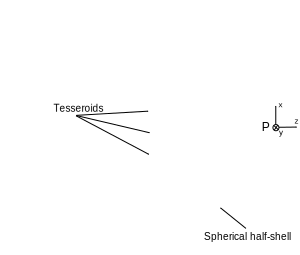
\includegraphics[width=\columnwidth]{figs/spherical-shell}
    \caption{A spherical half-shell
        spanning the ranges $0^{\circ} \le \lambda \le 180^\circ$,
        $-90^\circ \le \phi \le 90^\circ$,
        and $r_1 \le r \le r_2$,
        the corresponding tesseroid model,
        the computation point $P$
        at $(\lambda=90^\circ,\phi=0^\circ,r=r_2+h)$,
        and its local coordinate system $(x, y, z)$.
    }
    \label{fig:shell}
\end{figure}

For our comparison,
we used a spherical half-shell with
$\rho=2.7\ g.cm^{-3}$,
$r_1=6378.137\ km$ (mean Earth radius),
and
$r_2 = r_1 + 50\ km$.
We discretized the half-shell
into tesseroids of equal size
and calculated the gravitational effects of
the half-shell
(using equations \ref{eq:shellpot}-\ref{eq:shellgzz})
and the corresponding tesseroid model
at various heights.
These calculations were repeated
for varying values of
the distance/size ratio $R$.
This analysis
allows us to establish
the optimal value of $R$
that achieves a desired error level.

Data and source code to produce the results of this comparison
are provided by \textbf{(cite notebook on figshare)}.

\subsection{Software implementation}

The methods described above
were implemented the software package
Tesseroids version 1.1.1.
The package consists
of a range of command-line programs
written in the C programming language.
Tesseroids is free and open-source software
under the terms of
the 3-clause BSD license.

Each program performs a single type of calculation.
Programs receive input from
the standard input stream (\texttt{stdin})
and command-line arguments.
Output is made in plain text
through the standard output stream (\texttt{stdout}).

The main programs in Tesseroids are
\texttt{tesspot},
\texttt{tessgx},
\texttt{tessgy},
\texttt{tessgz},
\texttt{tessgxx},
\ldots ,
\texttt{tessgzz}
(henceforth referred to collectively as \texttt{tess*} programs).
These programs
calculate the gravitational potential,
gravitational attraction,
and Marussi tensor
caused by a tesseroid model.
The computation points are passed
through the standard input stream
and the tesseroid model
is passed through
a simple model file.
All programs receive
optional command-line arguments
that control the GLQ order (default is $N^\lambda=N^\phi=N^r=2$)
and distance/size ratio $R$
for the recursive division scheme.

The complete list of programs provided in Tesseroids is:

\begin{itemize}
    \item \texttt{tesspot}, \texttt{tessgx}, \texttt{tessgy}, \texttt{tessgz},
        \texttt{tessgxx}, \texttt{tessgxy}, \texttt{tessgxz},
        \texttt{tessgyy}, \texttt{tessgyz}, \texttt{tessgzz}:
        Calculate the gravitational potential, gravitational attraction,
        and Marussi tensor caused by a tesseroid model.
    \item \texttt{prismpot},
        \texttt{prismgx}, \texttt{prismgy}, \texttt{prismgz},
        \texttt{prismgxx}, \texttt{prismgxy}, \texttt{prismgxz},
        \texttt{prismgyy}, \texttt{prismgyz}, \texttt{prismgzz}:
        Calculate the gravitational potential, gravitational attraction,
        and Marussi tensor caused by a right-rectangular prism model
        in Cartesian coordinates
        using the formula of \citet{Nagy2000}.
    \item \texttt{prismpots}, \texttt{prismgs}, \texttt{prismggts}:
        Calculate the gravitational potential, gravitational attraction,
        and Marussi tensor caused by a right-rectangular prism model
        in spherical coordinates
        using the formula of \citet{Wild-Pfeiffer2008}.
    \item \texttt{tess2prism}: Converts a tesseroid model into
        right-rectangular prisms of equal mass.
    \item \texttt{tessgrd}: Generate regular grids.
    \item \texttt{tessdefaults}: Output the default values
        and values of physical constants used.
    \item \texttt{tessmodgen}: Generate a tesseroid model
        from a gridded relief (e.g., a digital elevation model).
    \item \texttt{tesslayers}: Generate a tesseroid model of
        a series of stacked layers.
    \item \texttt{tessmass}: Calculate the total mass of a tesseroid model.
\end{itemize}

Tesseroids is freely available
online\footnote{www.leouieda.com/tesseroids}.
\textbf{(cite archive on figshare)} provides a persistent
archive for the source code and compiled binaries of Tesseroids.


%%%%%%%%%%%%%%%%%%%%%%%%%%%%%%%%%%%%%%%%%%%%%%%%%%%%%%%%%%%%%%%%%%%%%%%%%%%%%%
\section{Results}

\begin{figure}
    \centering
    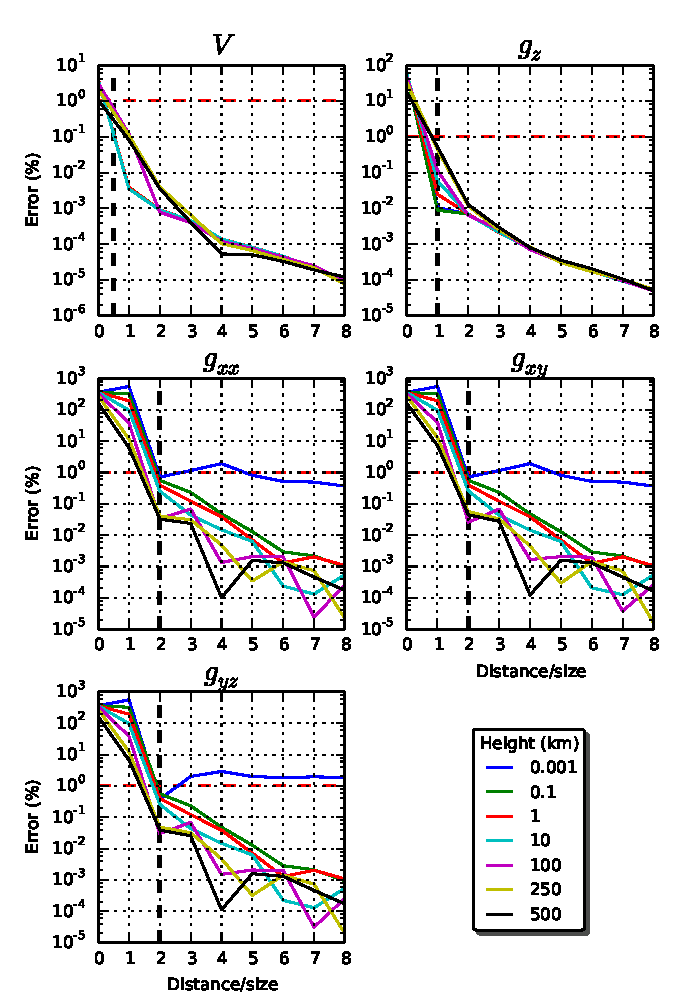
\includegraphics[width=\columnwidth]{figs/error-20deg}
    \caption{This is a figure caption.}
    \label{fig:error20}
\end{figure}

This is a reference to Figure \ref{fig:error20}.




%%%%%%%%%%%%%%%%%%%%%%%%%%%%%%%%%%%%%%%%%%%%%%%%%%%%%%%%%%%%%%%%%%%%%%%%%%%%%%
\section{Discussion}

%%%%%%%%%%%%%%%%%%%%%%%%%%%%%%%%%%%%%%%%%%%%%%%%%%%%%%%%%%%%%%%%%%%%%%%%%%%%%%
\section{Conclusions}

%%%%%%%%%%%%%%%%%%%%%%%%%%%%%%%%%%%%%%%%%%%%%%%%%%%%%%%%%%%%%%%%%%%%%%%%%%%%%%
\section{Acknowledgments}

Lorem ipsum dolor sit amet, consectetur adipiscing elit. Nam eu dolor pretium,
egestas mauris sed, dapibus quam. Duis hendrerit mollis nunc a consequat. Nulla
et sem consectetur, interdum velit eget, aliquam ipsum. Praesent sagittis
tortor diam, sed ultrices magna ullamcorper vitae. Proin vitae orci augue.
Morbi dictum ligula gravida sem malesuada facilisis. Mauris nibh metus, cursus
eget imperdiet vitae, pretium at lorem. Praesent nisi mauris, pretium ut risus
fermentum, egestas tincidunt nibh. Mauris nulla orci, consequat eu pharetra
non, mattis ut urna. Mauris facilisis orci eros. Nam mattis non magna iaculis
consectetur. Morbi sodales dolor vitae felis sagittis, eget faucibus turpis
convallis. Nullam malesuada, mauris et ultricies rutrum, odio nulla gravida
nunc, ac volutpat eros lectus eget lacus. Integer venenatis velit vel justo
pellentesque, quis molestie sem vestibulum.

\bibliographystyle{seg}
\bibliography{references}

\end{document}
